% \subsection{Structure Spatiale de l’ADN Procaryote}
% \label{sec:space_org}

% Dans la cellule, l'ADN ne reste pas sous cette forme primaire de séquence, il va se replier par différents mécanismes pour arriver dans une forme plus compacte qu'on appelle le chromosome (\autoref{fig:structure_dna}). L'ADN commence par se replier dans une structure secondaire, notamment la célèbre double hélice décrite par Watson, Crick et Franklin \cite{watson_molecular_1953}\footnote{Ces travaux sont souvent cités comme exemple dans la lutte pour la reconnaissance des femmes en sciences, Rosalind Franklin ayant joué un rôle essentiel, mais souvent sous-estimé dans cette découverte.}. Bien que la double hélice soit la forme la plus connue, d'autres conformations secondaires, telles que les structures en triple hélice ou en Z, ont également été identifiées, comme illustré dans la \autoref{fig:structure_dna}. L'organisation de l'ADN va au-delà de cette structure secondaire : il est ensuite soumis à des mécanismes de superenroulement induits par des enzymes spécifiques comme les topoisomérases et les gyrases. Ce superenroulement permet de réduire davantage la taille de l'ADN et de favoriser son organisation en boucles maintenues par des protéines structurales telles que HU, IHF ou H-NS \cite{williams_molecular_1997,prieto_genomic_2012}. Pour terminer, des protéines appelées histones vont terminer de replier l'ADN en formant des nucléosomes, les procaryotes utilisent ces protéines pour compacter leur ADN en une structure appelée nucléoïde. Cette forme, au-delà d'optimiser l'espace dans la cellule, permet aussi de stabiliser et de protéger l'ADN, ainsi que la régulation de l’expression des gènes. Par exemple, la méthylation de l’ADN, ainsi que les modifications des protéines associées, sont des mécanismes clés de l’épigénétique. Ces processus influencent la transcription des gènes et ont des implications fonctionnelles majeures. Des études récentes ont mis en lumière le rôle de la méthylation dans la régulation de la virulence bactérienne et dans la capacité des procaryotes à coloniser leurs hôtes \cite{oliveira_bacterial_2021}, soulignant ainsi l'importance de ces mécanismes dans la survie et l’adaptation des bactéries.

% \begin{figure}[htbp]
%     \centering
%     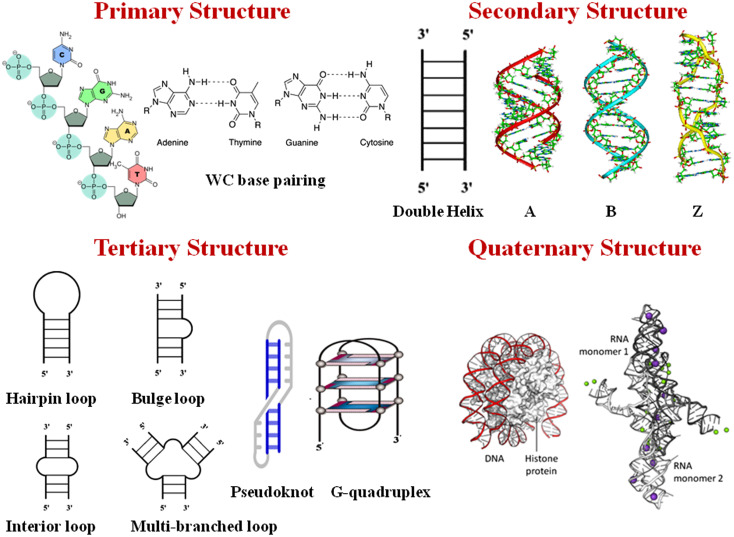
\includegraphics[width=0.8\linewidth]{images/structureDNA.jpg}
%     \caption[Structure de l'ADN]{Représentation de la structure primaire, secondaire, tertiaire et quaternaire d'un acide nucléique. PDB ID : 1EQZ et 4R4V. Tiré de \cite{kumar_biomolecular_2019}}
%     \label{fig:structure_dna}
% \end{figure}

% Un génome procaryote est donc sensible à la moindre modification dans la séquence d'ADN et l'expression des gènes directement répercuter sur les protéines présentent dans la cellule. Les protéines peuvent donc perdre leur capacité à fonctionner correctement, soit ne pas être produite du tout. Une vision plus positive sera aussi d'imaginer que des changements dans la séquence d'ADN permettrons de produire une nouvelle protéine d'intérêt pour la cellule. Dans la suite, avec une vision darwinienne\footnote{Vision de l'évolution proposée par Charles Darwin, qui propose que les espèces évolue perpétuellement de façon hasardeuse et que les innovations génétiques sont ensuite maintenues ou perdues dans les populations par pression de sélection}, nous verrons par quels mécanismes la séquence d'ADN va évoluer, mais aussi comment ces évolutions seront transmises aux autres cellules procaryotes. 
